% !TEX program = pdflatex+makeindex+bibtex
% !TEX encoding = UTF-8 Unicode
% !TEX spellcheck = de_ch

% created by Simon Schälli <simon.schaelli@kantiwattwil.ch>
% v1.0 ursprüngliche Version
% v1.1 2015-10-22 mit Titelbild
% v1.2 2016-09-30 aufgeräumt
% v1.3 2016-10-16 Layoutfehler behoben

%======================================================================%
%=== Dokument auf häufige Fehler überprüfen                         ===%
%======================================================================%
\RequirePackage[l2tabu, orthodox]{nag}

%======================================================================%
%=== Dokumentklasse wählen                                          ===%
%======================================================================%
\documentclass[a4paper
,openright]{scrreprt}

%======================================================================%
%=== Pakete einbinden                                               ===%
%======================================================================%
\usepackage[utf8]{inputenc}
\usepackage[ngerman]{babel}
\usepackage{geometry}
\geometry{a4paper, top=25mm, bottom=30mm, headsep=10mm, footnotesep=12mm}

% Latin Modern Schriftart
\usepackage{lmodern}
\usepackage[T1]{fontenc}

% Mathematik-Pakete
\usepackage{amsmath}
\usepackage{amssymb}

% mathematische Buchstaben als Text
\usepackage{textcomp}

% komfortable Referenzen mit \fref
\usepackage[german]{fancyref}

% Kopf- und Fusszeilen
\usepackage[automark,headsepline]{scrpage2}
\ihead[]{\headmark}
\chead[]{}
\ohead[]{\pagemark}
\ifoot[]{}
\cfoot[\pagemark]{}
\ofoot[]{}

% Einfügen von Bildern
\usepackage{graphicx}

% schöne Tabellen
\usepackage{booktabs}

% Tabelleninhalt an Dezimalpunkt ausrichten
\usepackage{dcolumn}
\makeatletter                     % <- hebt Sonderbedeutung von @ auf
\newcolumntype{d}[1]{D{.}{.}{#1}} % <- definiert einen neuen Spaltentyp
\makeatother                      % <- setzt Sonderbedeutung von @ wieder

% Beispieltext
\usepackage{lipsum}

% Hyperlinks in PDF
\usepackage{hyperref}

%======================================================================%
%=== Angaben zum Dokument                                           ===%
%======================================================================%


\titlehead{Beuth Hochschule für Technik Berlin \hfill Inga Schwarze\\
Fachbereich VI \hfill Tegeler Weg 107\\
Informatik und Medien \hfill 10589 Berlin\\
Studiengang Medieninformatik, 7. Semester \vspace{2cm}}
\title{Praxisbericht}
\subtitle{über das Praktikum in der Wall GmbH}
\author{\texorpdfstring{von Inga Schwarze\\Matrikelnummer: 820789\\ [5mm] \small Hochschulbetreuung: Prof. Dr. Sven Graupner\\ \small Betriebliche Betreuung: Mario Russo \& Dipl. Inf. (FH) Jörg Biallas \\ [1cm]
\includegraphics[scale=0.2]{figures/beuthlogo}\\ [1cm] \includegraphics[scale=0.2]{figures/WALL-AG} \\}{Inga Schwarze}}
\date{\small Wall GmbH \\ Friedrichstraße 118 \\ 10117 Berlin \\ [5mm] \textbf{Zeitraum: 01.08.17 - 31.10.17}\\ \vspace{5mm}}

%======================================================================%
%=== PDF Dokumenteinstellungen                                      ===%
%======================================================================%

\makeatletter
\hypersetup{
	pdftitle={\@title},%
	pdfsubject={\@subject},%
	pdfauthor={\@author},%
	pdfkeywords={},%
	colorlinks,%
	citecolor=black,%
	filecolor=black,%
	linkcolor=black,%
	urlcolor=black}%
\makeatother

%======================================================================%
%=== Beginn des eigentlichen Dokumentes                             ===%
%======================================================================%

\begin{document}

\maketitle % <- Titel setzen
\cleardoublepage
\pagenumbering{arabic} % <- römische Seitennummerierung
\tableofcontents % <- Inhaltsverzeichnis
\cleardoublepage % <- neue Seite

% Kapitel einbinden:
% !TEX root = ../praktikumsbericht.tex
\chapter{Praktikumsbetrieb}\label{chap:praktikumsbetrieb}
\section{Wall GmbH}\label{sec:wallgmbh}

„Die Wall GmbH ist ein deutsches Unternehmen mit Sitz in Berlin, das sich auf die Entwicklung und Produktion von Stadtmöbeln und die Vermarktung hinterleuchteter Werbeflächen spezialisiert hat.“\footnote{\label{foot:1}Wikipedia: „Wall GmbH“, unter: http://de.wikipedia.org/wiki/Wall\_GmbH (abgerufen am 03.12.2017)} Seit 2009 ist die Wall GmbH Teil der internationalen JCDecaux-Gruppe, der Nummer 1 der Außenwerbung weltweit. JCDecaux erzielte im Jahr 2015 einen Umsatz von 3.207 Millionen Euro in mehr als 60 Ländern mit 12.850 Mitarbeitern, von denen mehr als 1.000 Mitarbeiter zur Wall GmbH zählen.\footnote{\label{foot:2}Wall GmbH: „Fakten“, unter: http://www.wall.de/de/company/facts (abgerufen am 03.12.2017)} Die Wall GmbH bietet Städten im Rahmen von Stadtverträgen individuell konzipierte Stadtmöbel an, die sie kostenfrei installiert, reinigt und wartet. Das Unternehmen refinanziert die kostenfreien Produkte und Dienstleistungen über die Vermarktung der in die Stadtmöbel integrierten Werbeflächen. Darüber hinaus werden die Städte an den Einnahmen der Außenwerbung beteiligt.\footnote{\label{foot:3}Berliner Morgenpost: „Berliner Wall AG will sich komplett digital aufstellen“, unter: https://www.morgenpost.de/berlin/article132236230/Berliner-Wall-AG-will-sich-komplett-digital-aufstellen.html (abgerufen am 06.01.2018)} \\ Das Unternehmen möchte mit seinen hochwertigen Produkten die Informations- und Lebensqualität für die Bürger und Besucher der Städte im öffentlichen Raum verbessern. Das Angebot erstreckt sich von leistungsstarken Werbenetzen über U-Bahnhöfe bis hin zu Transportmitteln. Insgesamt vermarktet die Wall GmbH in Deutschland mehr als 76.000 Werbeflächen (Stand: 31. Dezember 2016).\footnote{\label{foot:4}Wall GmbH: „Fakten“, unter: http://www.wall.de/de/company/facts (abgerufen am 06.01.2018)} 

\subsection{Unternehmenskonzept}\label{sec:unternehmenskonzept}
Wall setzt, im Gegensatz zu seinem großen Konkurrenten \textit{Ströer}, auf das Konzept „Alles aus einer Hand“. Die Stadtmöbel entstehen in einem eigenen Forschungs- und Entwicklungszentrum in Velten bei Berlin. In dem eigenen Produktionswerk verspricht Wall nicht nur höchste Design- und Materialqualität, sondern bietet den Städten entsprechend ihren spezifischen Anforderungen maßgeschneiderte Lösungen.\footnote{\label{foot:5}Vgl. ebd.} \\ Getreu dem Motto „Für Städte. Für Menschen.“ versteht sich Wall als Partner der Städte. Werbetreibenden soll eine innovative mediale Vielfalt zur Übermittlung ihrer Botschaft angeboten werden.\footnote{\label{foot:6}Wall GmbH: „Philosophie“, unter: http://www.wall.de/de/company/philosophy (abgerufen am 07.01.2018)} 

\subsection{Unternehmensbereiche}\label{sec:unternehmensbereiche}
Das Unternehmen gliedert sich in vier Unternehmensbereiche: Forschung \& Entwicklung, Produktion, Vermarktung und Reinigung \& Wartung. \\ Die Abteilung der Forschung und Entwicklung arbeitet daran, in Sachen Stadtmöblierung und Außenwerbung innovative, nachhaltige und kreative Lösungen zu schaffen. \\ In der Produktion hat die Präzision in der Fertigung oberste Priorität. Das Produktionswerk in Velten ist eines der modernsten Europas. Auf 10.000 qm arbeiten dort qualifizierte Mitarbeiter mit ausgefeilter Technik und hochwertigen Materialien. \\ Zum Bereich Reinigung und Wartung gehören ausschließlich eigens geschulte Mitarbeiter und ein ausgefeiltes Wartungs- und Reinigungskonzept. Dadurch kann gewährleistet werden, dass die Produkte jederzeit einwandfrei funktionieren und aussehen. Außerdem sind alle Produkte mit modernster Überwachungstechnik ausgestattet. Eine 24h-Hotline stellt sicher, dass Reparaturen umgehend ausgeführt werden können.\footnote{\label{foot:7}Wall GmbH: „Unternehmensbereiche“, unter: http://www.wall.de/de/company/unternehmensbereiche (abgerufen am 07.01.2018)} \\ Auf den Unternehmensbereich der Vermarktung gehe ich im nächsten Abschnitt ein. 

\subsection{WallDecaux}\label{sec:walldecaux}
Mein Praktikum ist im Unternehmensbereich der Vermarktung angesiedelt. In Deutschland wird das gemeinsame Portfolio von JCDecaux und der Wall GmbH unter der Vertriebsmarke „WallDecaux Premium Out of Home“ vermarktet. WallDecaux bündelt die Stärken der beiden familiengeführten Unternehmen, die beide in den vergangenen Jahrzehnten die Professionalisierung der Außenwerbung maßgeblich gestaltet haben.\footnote{\label{foot:8}Wall GmbH: „WallDecaux“, unter: http://www.wall.de/de/outdoor\_advertising/walldecaux (abgerufen am 07.01.2018)} \\ Durch die Zusammenführung der beiden Vertriebsbereiche ist WallDecaux zum Beispiel der größte Anbieter in Deutschland für das Format „City Light Poster“ und misst rund 49.000 CLP-Werbeflächen in mehr als 30 Städten.\footnote{\label{foot:9}Vgl. ebd. (abgerufen am 07.01.2018)} 

\section{Weg zur Praktikumsstelle}\label{sec:wegzurstelle}
Wenige Monate vor Beginn meines Praktikums suchte ich bereits nach einer neuen beruflichen Herausforderung, die zu meinen Interessensschwerpunkten und meiner Studienwahl passte. Dabei wurde ich auf die Wall GmbH aufmerksam und bewarb mich dort als Werkstudentin. Nach einem aufschlussreichen Bewerbungsgespräch, das mein Interesse weiter verstärkte, erhielt ich die Job-Zusage und arbeitete ab diesem Zeitpunkt als studentische Hilfskraft im digitalen Marketing der Wall GmbH. Sofern sich auch für den Zeitraum des Praktikums ein geeigneter Aufgabenbereich für mich finden ließe, standen mein Team und ich dieser Idee sehr aufgeschlossen gegenüber. \\ Als während meiner Einarbeitung als Werkstudentin klar wurde, dass es einen hohen Bedarf an Schnittstellentätigkeiten zwischen der IT-Abteilung und dem Marketing gibt, entschied ich mich, die Herausforderung anzunehmen und diese Aufgaben in einem dreimonatigen Vollzeitpraktikum auszuüben. Es bot sich dadurch für mich die Chance, einen Einblick in gleich zwei Unternehmensbereiche erhalten zu können. Die Interaktion zwischen IT-bezogenen Aufgabenbereichen und multimedialen (Kreativ-)Prozessen war für mich schon immer von großem Interesse und ausschlaggebend für meine berufliche Zukunft. In beiden Aufgabenfeldern sehe ich meine persönlichen Stärken, sodass dieses Praktikum mit Sicherheit Aufschluss über einen möglichen Berufswunsch geben und eine Rolle bei der späteren Berufswahl spielen würde. 

\newpage
% !TEX root = ../praktikumsbericht.tex
\chapter{Tätigkeitsbereiche und Aufgaben}\label{chap:aufgaben}

Wie bereits erwähnt, hat sich schon zu meiner Zeit als Werkstudentin bei Wall herausgestellt, dass es einige Schnittstellentätigkeiten zwischen der IT-Abteilung und dem Marketing gibt, bei denen mein Team aus dem digitalen Marketing Unterstützung gebrauchen könnte. Vor dem Hintergrund, dass diese Bereiche durch den digitalen Wandel zunehmend miteinander verschmelzen, werden die Aufgaben oft komplexer und die Klärung des Zuständigkeitsbereichs gestaltet sich schwieriger. An diesem Punkt setzt mein Praktikum an: ich sollte Arbeitsaufträge erhalten, die sowohl im Digitalen Marketing, als auch in der IT Anwendung finden, denn dort ist Zusammenarbeit Pflicht. \\ Da sich meine Aufgabenbereiche als sehr vielfältig herausgestellt haben und es keine große Kernaufgabe gab, an der ich für drei Monate arbeiten sollte, geben die folgenden Abschnitte einen Einblick in die Arbeitsbereiche, mit denen ich mich am meisten beschäftigte. 

\section{Einarbeitung}\label{sec:einarbeitung}

Zu Beginn meines Praktikums wurde ich zunächst allen Personen aus dem Marketing und der IT-Abteilung vorgestellt, mit denen ich künftig zusammenarbeiten würde. Insgesamt empfand ich es als sehr aufmerksam und respektvoll, wie man mich an die verschiedenen Themenbereiche heranführte. Für die Einarbeitung nahmen sich meine Betreuer stets viel Zeit und legten Wert darauf, mich mit den jeweiligen Tools intensiv vertraut zu machen. Neben einer eigenen E-Mail-Adresse erhielt ich auch eigene Accounts und Zugänge für den alten und neuen Webseiten-Bereich sowie für das Intranet. Zusätzlich erhielt ich einige hausinternen, aber auch externen Infomaterialien zum Unternehmen und dem dazugehörenden Portfolio. \\ Da ich mit verschiedenen Tools und Content-Management-Systemen arbeiten würde, hat die Einarbeitungsphase möglicherweise mehr Zeit eingenommen, als vorher angenommen. Zur Einarbeitung erhielt ich meistens kleinere, nicht zeitgebundene Aufgaben; z.B. das Austauchen von Kontakten und Bildern auf der aktuellen Webseite oder die Aktualisierung von Daten im Intranet. Nachdem mir die grundlegende Funktionsweise der Systeme nähergebracht wurde, konnte ich viele Aufgaben nach dem \textit{Learning by Doing}-Prinzip bewerkstelligen, was mich stets motiviert und einen großen Lerneffekt zur Folge hatte. \\ Obwohl ich zu Beginn meines Praktikums schon seit drei Monaten im Unternehmen arbeitete, erwies sich die Einarbeitungsphase als angemessen, da viele Aufgabenfelder für mich noch neu waren. Trotzdem waren die drei vorangegangenen Monate als Werkstudent hilfreich, um mich einzugewöhnen und die wichtigsten Strukturen und Konzepte des Unternehmens zu verstehen. 

\section{Website Relaunch}\label{sec:webrelaunch}

Den wohl größten und intensivsten Teil meines Praktikums nimmt der Relaunch der Website von Wall ein. Das neue Website-Konzept und Redesign von wall.de beschäftigte mich während der gesamten Praktikumszeit. Da mein Team fast ausschließlich am Website-Projekt arbeitete, dienten viele meiner anderen Aufgabenbereiche dazu, das Team dahingehend zu entlasten. Dadurch bot sich für mich die Möglichkeit, sowohl an einem großen Vorhaben mitwirken zu können, als auch andere Teilbereiche abzudecken und kennenzulernen. \\ Zu Beginn meines Praktikums arbeitete mein Team bereits seit über einem Jahr an der neuen Website und ich stieg somit zu einem Zeitpunkt in das Projekt ein, an dem große Teile des Konzepts bereits feststanden und auch ein Teil des Contents schon eingebunden wurde. \\ Meine Aufgabe war es nun, bei der Gestaltung und der Konzeptionierung der noch offenen Seiten mitzuhelfen: Von der Idee über ein Konzept und den Entwurf bis hin zur Umsetzung mit Blick auf das Front-End wurde ich in alle Prozesse einbezogen. \\ Die neue Website wurde mit dem Content-Management-System und Framework Drupal entwickelt. Die Entscheidung, mit diesem CMS zu arbeiten, wurde nicht innerhalb unserer Abteilung getroffen, sondern entspricht den Rahmenbedingungen von JCDecaux weltweit. Als Teil dieses internationalen Unternehmens war es das Ziel, sich am Look \& Feel der offiziellen Website von jcdecaux, \textit{www.jcdecaux.com} zu orientieren und daher mit demselben Framework zu arbeiten. Ok cool


\section{Event Management}\label{sec:eventmanagement}
\section{Sonstige Aufgaben}\label{sec:sonstiges}
\section{Praktikum und Studium}\label{sec:praktikumstudium}
\subsection{Wissensanwendung im Praktikum}\label{sec:wissensanwendung}
\subsection{Bedeutung für die Zukunft}\label{sec:zukunft}

\newpage
% !TEX root = ../praktikumsbericht.tex
\chapter{Bewertung des Praktikums}\label{chap:bewertung}
Darlegung des Methodenansatzes.
\newpage
% !TEX root = ../maturaarbeit.tex
\chapter{Ergebnisse}\label{chap:ergebnisse}
Die Ergebnisse einer anderen Arbeit sind in \cite{Boney96} dokumentiert.
\LaTeX-Dateien können auch einfach per \verb+\input{pfad/zum/dokument.tex}+ eingebunden werden, so wie dies mit \fref{tab:tabelle2} geschehen ist.
% !TEX root = ../maturaarbeit.tex
\begin{table}[th]
  \centering
  \footnotesize
  \caption{Anwendung von Linien}
  \label{tab:tabelle2}
  \begin{tabular}{@{}l*{4}{d{4.0}}@{}}
    \toprule
      Monat & 1965 & 1966 & 1967 & 1968 \\
    \cmidrule(r){1-1}\cmidrule(lr){2-2}\cmidrule(lr){3-3}\cmidrule(lr){4-4}%
      \cmidrule(l){5-5}
      November  & 2500 & 2800 & 4700 & 3200 \\
      Dezember  & 2300 & 2000 & 3600 & 2700 \\
    \bottomrule
  \end{tabular}
\end{table}
Einige andere Ergebnisse finden sich in \fref{tab:tabelle1}.\\
Wenn man \LaTeX\ nicht zu fest dreinredet, macht es was es soll.

\begin{table}
  \centering
  \caption[CUDA Messdaten]{Ein paar CUDA Messdaten}
  \label{tab:tabelle1}
  \footnotesize
  \begin{tabular}{@{}ld{3.0}*{2}{d{4.2}}d{2.2}@{}}
    \toprule
    \multicolumn{0}{@{}l}{Method} & \multicolumn{1}{c}{\# Calls} & \multicolumn{1}{c}{GPU time [\textmu s]} & \multicolumn{1}{c}{CPU time [\textmu s]} & \multicolumn{1}{c@{}}{GPU time [\%]}\\
    \midrule
    sumvecel\_kernel&386&3095.55&3613.56&19.84\\
    matvec\_kernel&193&2587.87&2848.87&16.58\\
    mattransvec\_kernel&193&2566.69&2792.69&16.45\\
    scalvec\_kernel&386&2322.11&2778.11&14.88\\
    squarevecel\_kernel&386&2098.62&2547.62&13.45\\
    sasum\_gld\_main&193&2044.48&2299.48&13.10\\
    memcpyDtoH&202&831.52&3632.52&5.32\\
    memcpyHtoD&7&28.54&36.54&0.18\\
    sger\_main\_hw&3&27.04&30.04&0.17\\
    \bottomrule
  \end{tabular}
\end{table}
\newpage
% !TEX root = ../maturaarbeit.tex
\chapter{Diskussion}\label{chap:diskussion}
Diskussion der Messdaten...

\section{Eine Figur}\label{sec:eine figur}
In \fref{fig:matlabfigur} kann man schöne Farben erkennen. Im Gegensatz dazu sehen die Formeln aus \fref{sec:ueber einstein} ein bisschen blass aus. Man erkennt auch eine gewisse Grösse von \LaTeX, Referenzen zu setzen.
\begin{figure}[ht]
	\centering
	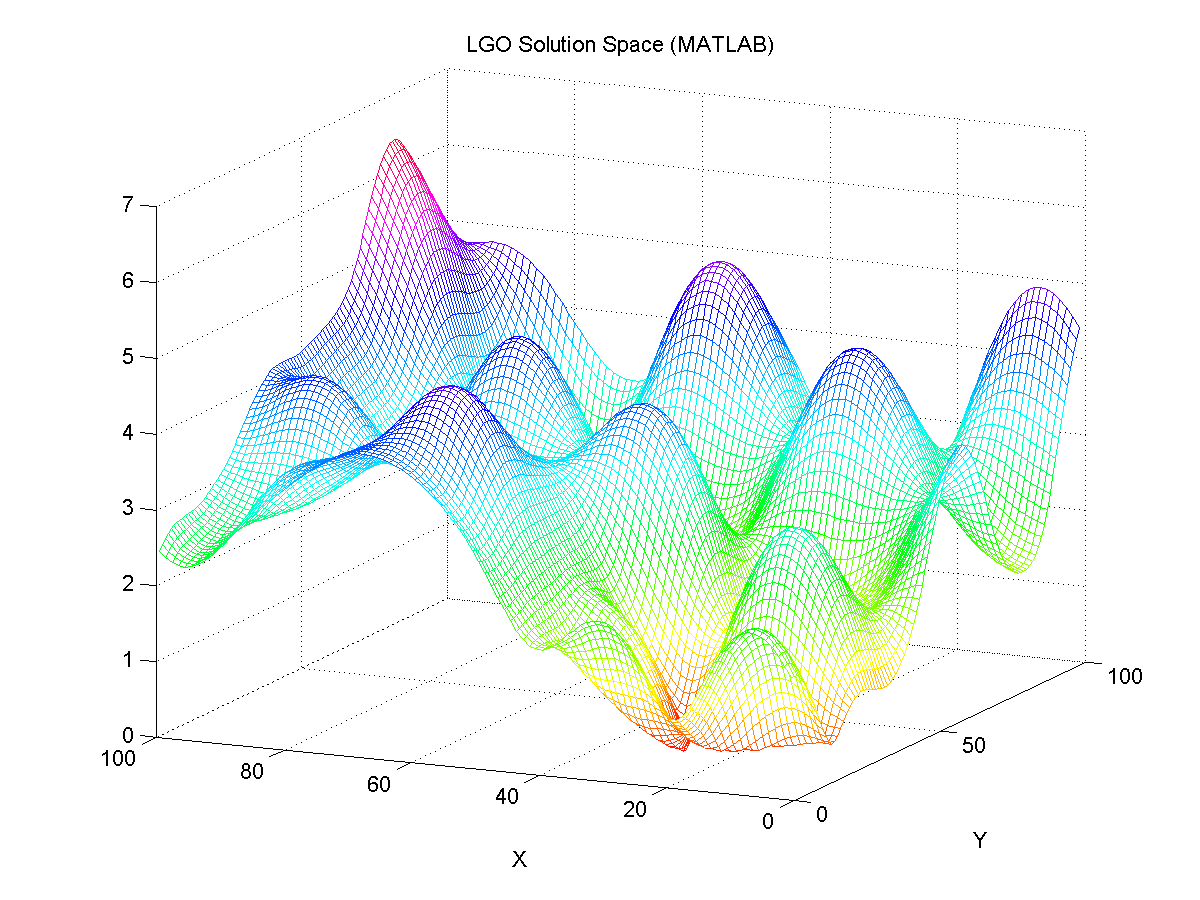
\includegraphics[scale=0.3]{figures/matlabgraph}
	\caption[MATLAB Plot]{Ein Plot aus dem Internet \cite{Plot}, der mit MATLAB erstellt wurde.}
	\label{fig:matlabfigur}
\end{figure}

\newpage
% !TEX root = ../maturaarbeit.tex
\chapter{Schluss}\label{chap:schluss}
\begin{enumerate}
	\item Kurze, prägnante Zusammenfassung der Ergebnisse, In-Beziehung-Stellen der Ergebnisse zur Einleitung
	\item Anregungen zur weiteren Vertiefung
Persönliche Bemerkungen: Schlussfolgerungen
	\item Welche neuen Erkenntnisse? Wo zeigten
sich besondere Schwierigkeiten? usw.
\end{enumerate}

\newpage

\appendix % <- Anhang
\listoffigures % <- Abbildungsverzeichnis
\listoftables  % <- Tabellenverzeichnis
% !TEX root = ../maturaarbeit.tex
\begin{thebibliography}{20}% 100 is a random guess of the total number of
%references
\bibitem{Boney96} Boney, L., Tewfik, A.H., and Hamdy, K.N., ``Digital
Watermarks for Audio Signals," \emph{Proceedings of the Third IEEE
International Conference on Multimedia}, pp. 473-480, June 1996.
\bibitem{MG} Goossens, M., Mittelbach, F., Samarin, \emph{A LaTeX
Companion}, Addison-Wesley, Reading, MA, 1994.
\bibitem{HK} Kopka, H., Daly P.W., \emph{A Guide to LaTeX},
Addison-Wesley, Reading, MA, 1999.
\bibitem{Pan} Pan, D., ``A Tutorial on MPEG/Audio Compression," \emph{IEEE
Multimedia}, Vol.2, pp.60-74, Summer 1998.
\bibitem{Plot} \url{http://tugll.tugraz.at/39093/files/-1/758/matlabgraph.gif}
\end{thebibliography} % <- Literaturverzeichnis

\end{document}